\documentclass{article}

\usepackage{fancyhdr}
\usepackage{ragged2e}
\usepackage{graphicx}
\usepackage{caption}
\usepackage{geometry}
\usepackage{amsmath}
\usepackage{rotating}

\usepackage{listings}
\usepackage{color}

\definecolor{dkgreen}{rgb}{0,0.6,0}
\definecolor{gray}{rgb}{0.5,0.5,0.5}
\definecolor{mauve}{rgb}{0.58,0,0.82}

\lstset{frame=tb,
  language=Java,
  aboveskip=3mm,
  belowskip=3mm,
  showstringspaces=false,
  columns=flexible,
  basicstyle={\small\ttfamily},
  numbers=none,
  numberstyle=\tiny\color{gray},
  keywordstyle=\color{blue},
  commentstyle=\color{dkgreen},
  stringstyle=\color{mauve},
  breaklines=true,
  breakatwhitespace=true,
  tabsize=4
}

\setcounter{secnumdepth}{1}

\usepackage{chngcntr}
\counterwithin{figure}{section}

\renewcommand*{\thepage}{C\arabic{page}}

\pagestyle{fancy}
\lhead{ACME Robotics}
\chead{\#8367}
\rhead{\ifcontents Contents \else Week \thesection \fi}

\newif\ifcontents
\contentstrue

\makeatletter
\renewcommand{\@seccntformat}[1]{}
\makeatother

\begin{document}\contentsfalse

 
\subsection{Sorter Finalization}
%! Complete last edits to the sorter.
The sorter needed to be printed as soon as possible so Ashlin and Aidan made some finalizing touches to the sorter so that it could print. First they split it the base design into two parts making the top be its own piece. They did this so that the top could be removed to allow for the swiveler to be put in the sorter and also so that the top piece could be printed separately to allow for the print to be easier. They also edited the top piece so that a bearing could fit into it tightly which would allow for the overall rotation of the sorter to be that much smoother. They printed the sorter on one of their sponsor's printers (see Figure \ref{}).

\begin{figure}
    \centering
    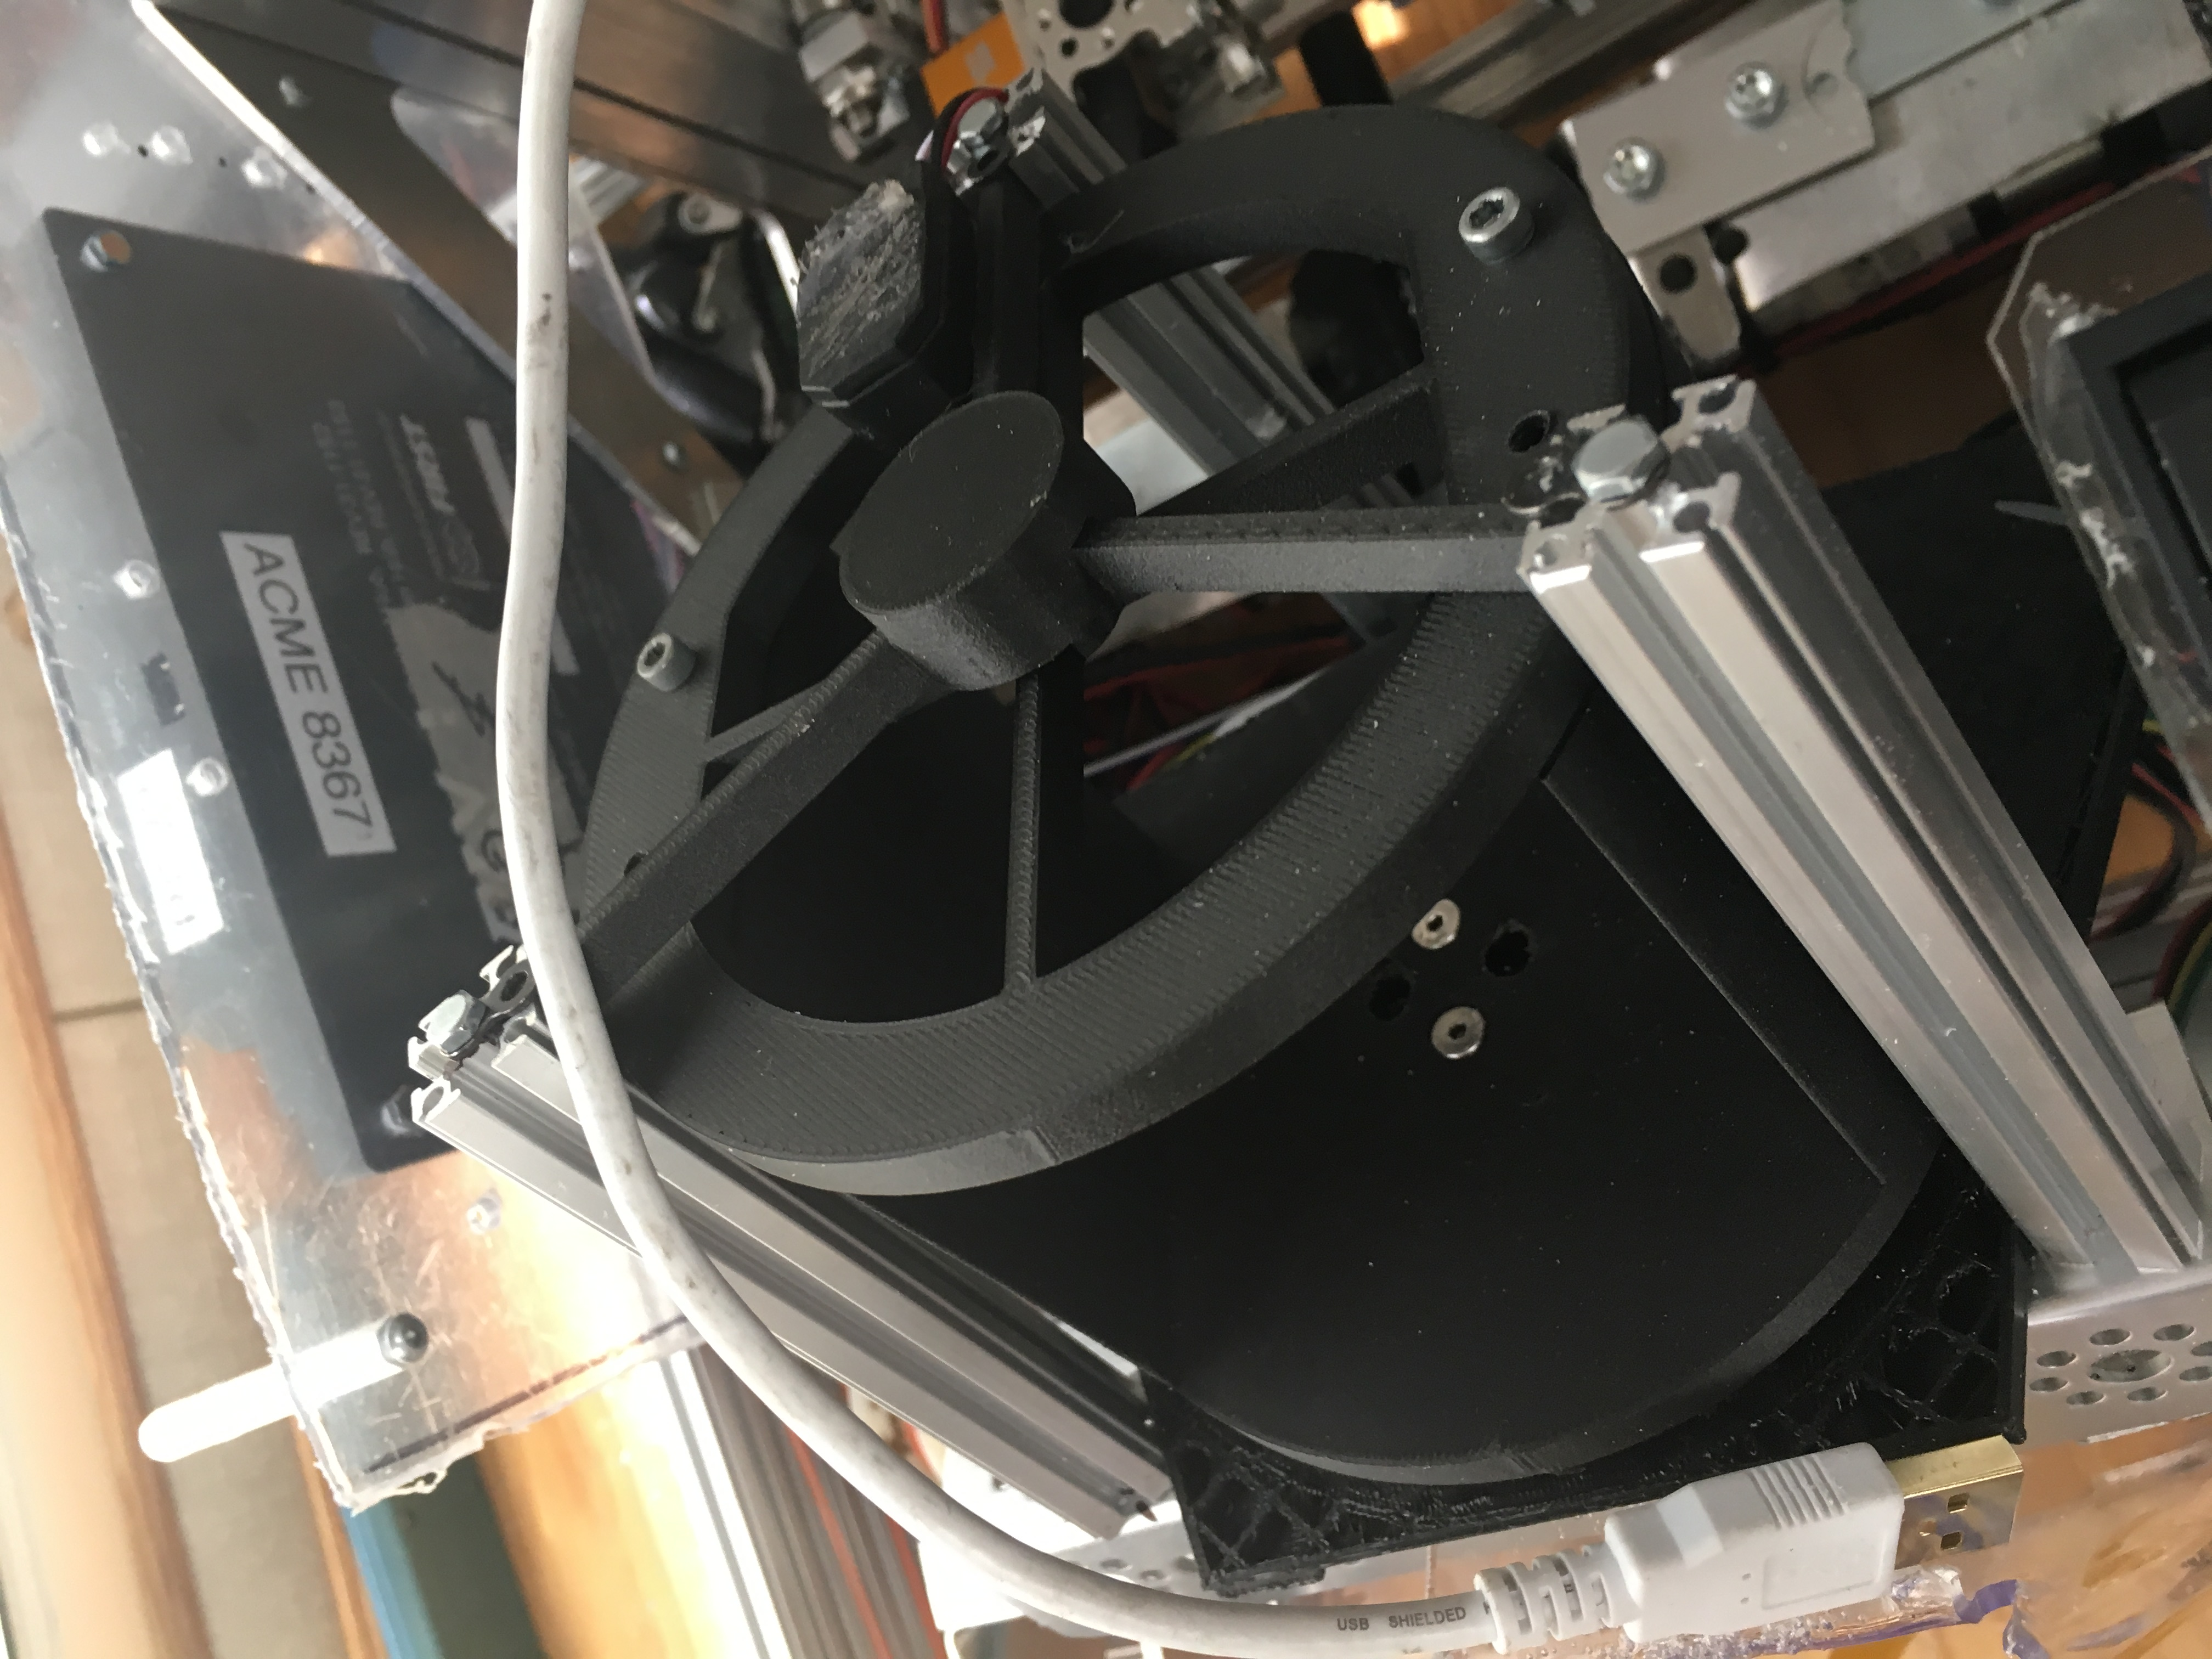
\includegraphics[width=.6 \textwidth, angle=270 ]{10_11-05/images/sorter.JPG}
    \caption{Sorter and Intake CAD}
    \label{fig:Intake CAD}
\end{figure}

\subsection{Intake shield}
%! Manufacture and make intake shield.
After the intake shield was cut Ashlin and Aidan heat bent the shield so that it would be shaped exactly as the 3D model. After the shield was bent they tested it to make sure it successfully in-took balls and cubes. The testing was successful and the shield worked  spectacularly.

\begin{figure}
    \centering
    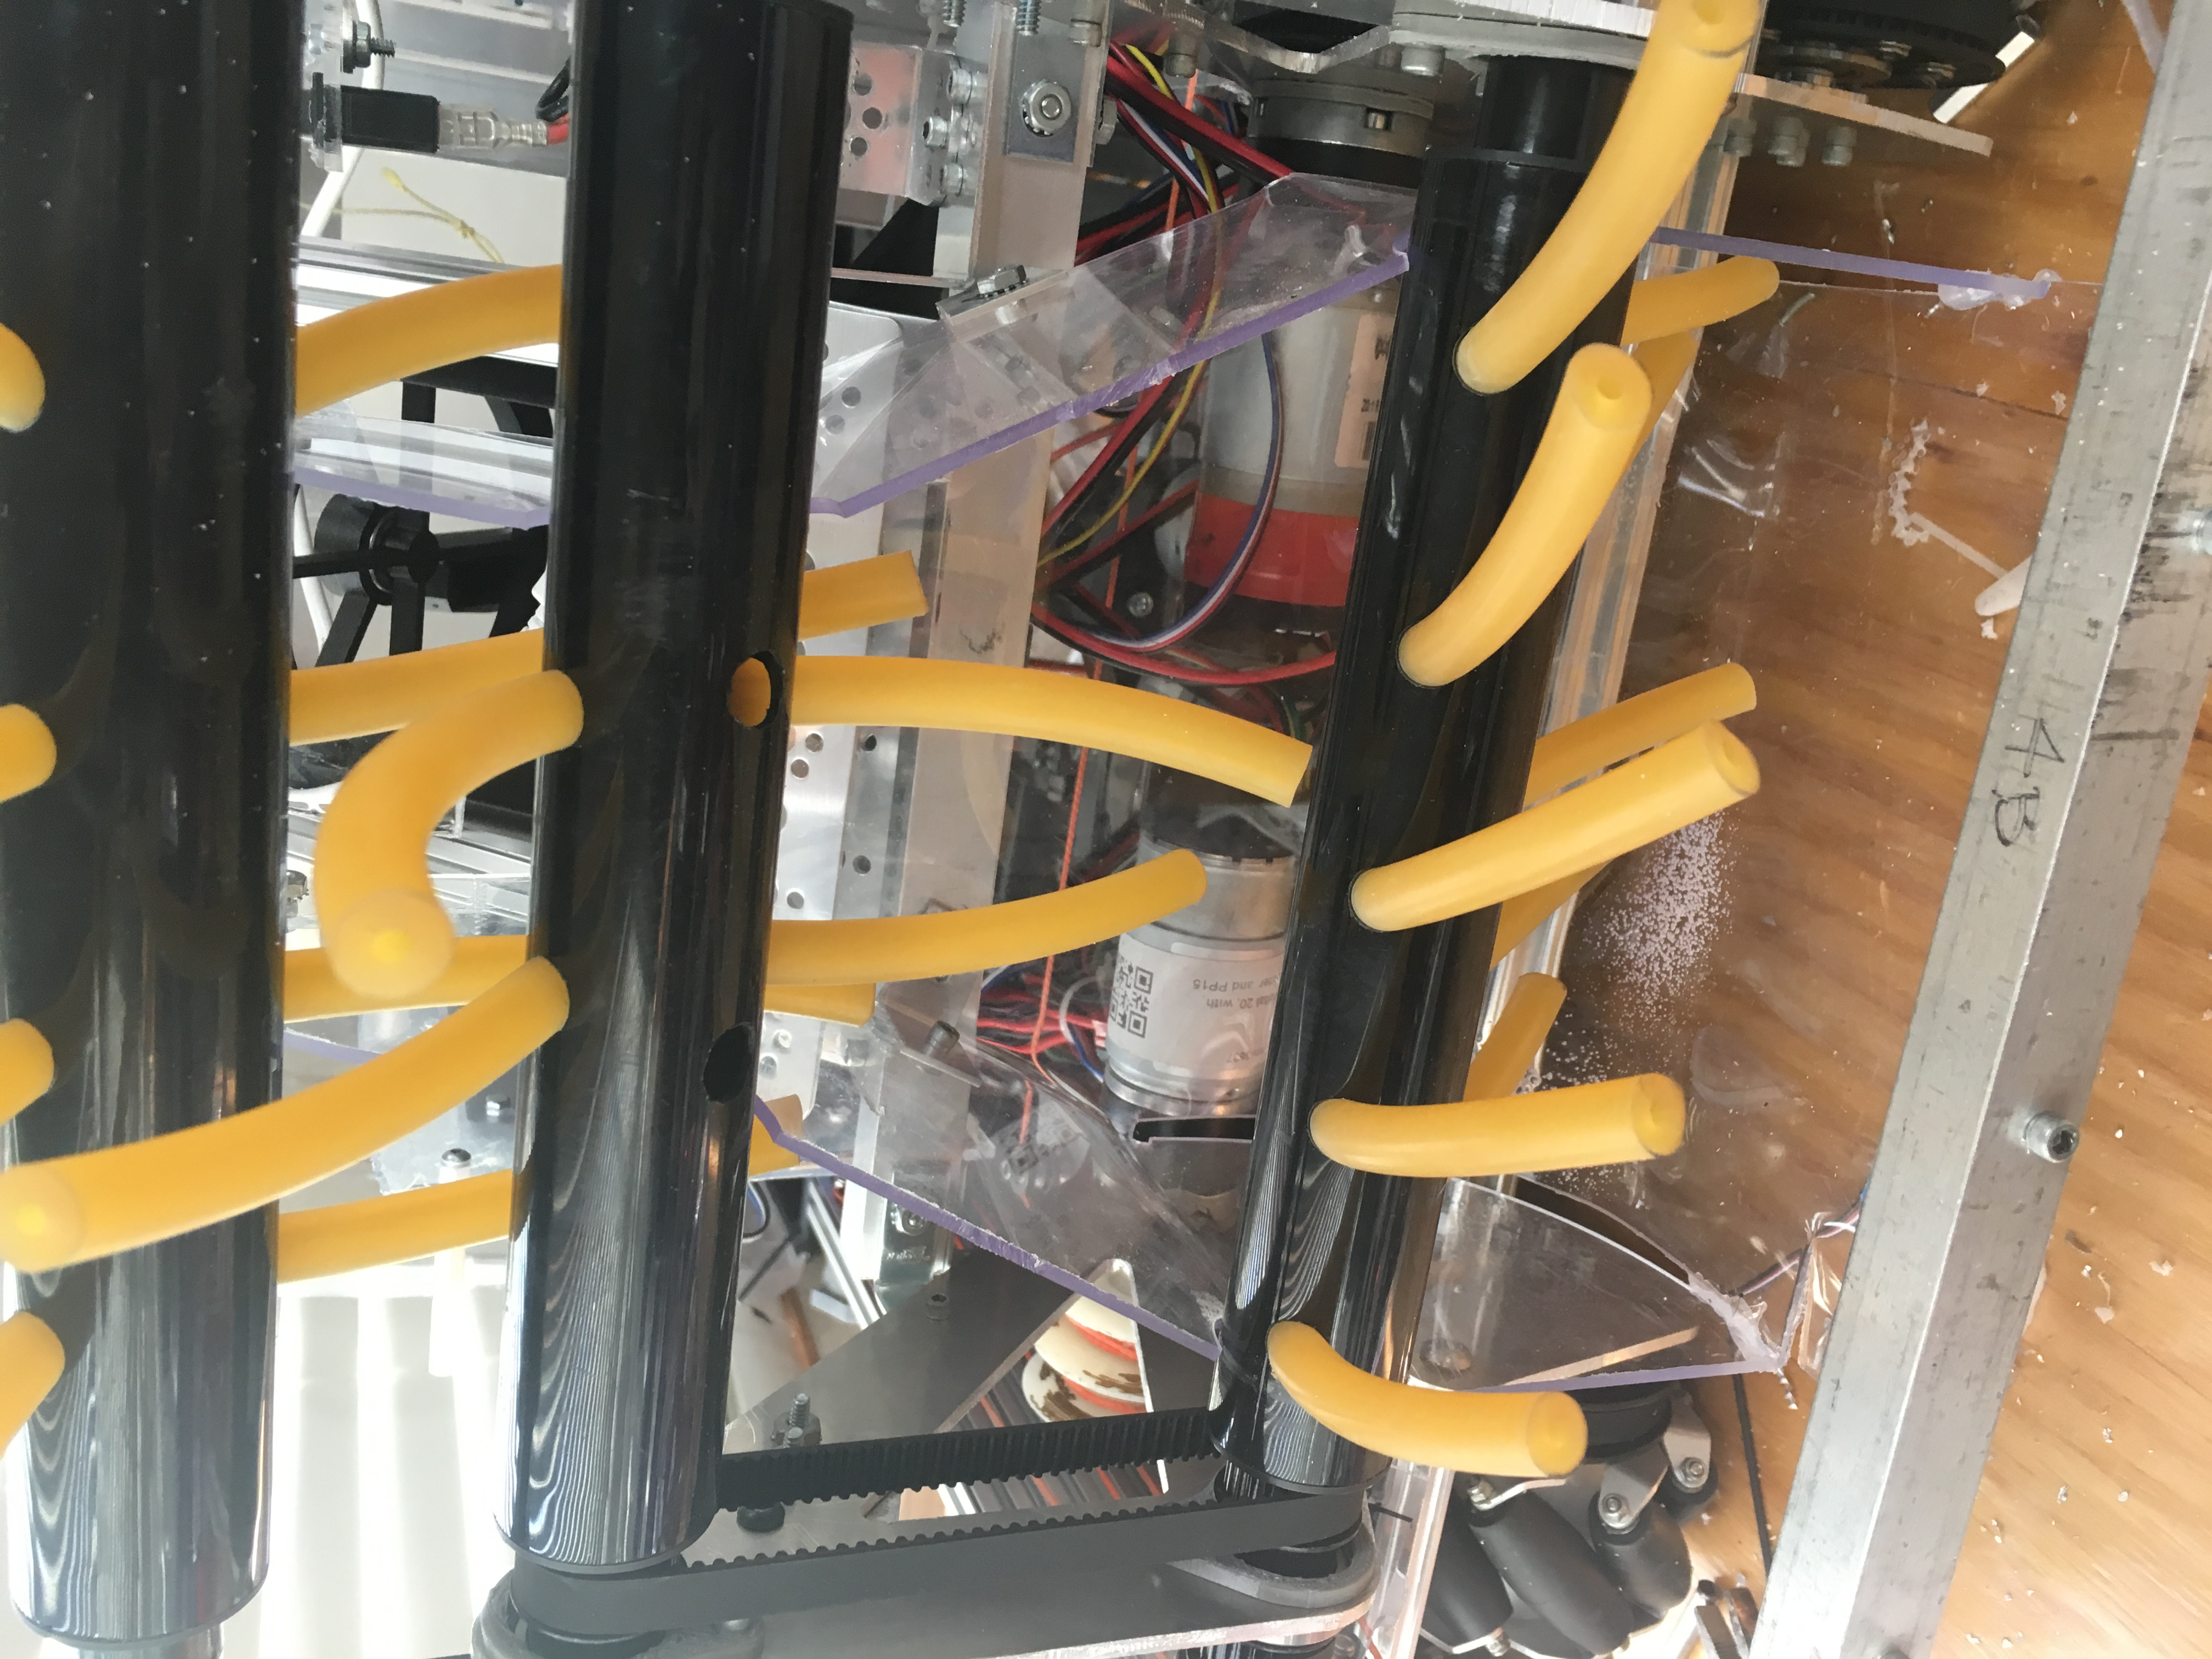
\includegraphics[width=.6\textwidth, angle=270]{10_11-05/images/intake_shield.JPG}
    \caption{Intake Shield}
    \label{fig:Intake Shield}
\end{figure}

\subsection{Drivetrain Assembly}
%! Assemble the drivetrain.
This week Oren assembled all of the parts for the drive-train, there was some errors and misshapes. That include needed motor mounts, new more accurately cut cross members and some needed   screw holes for mounting things. The drive-train when completed functioned actually like we had planned and was very silent when running.    

\begin{figure}
    \centering
    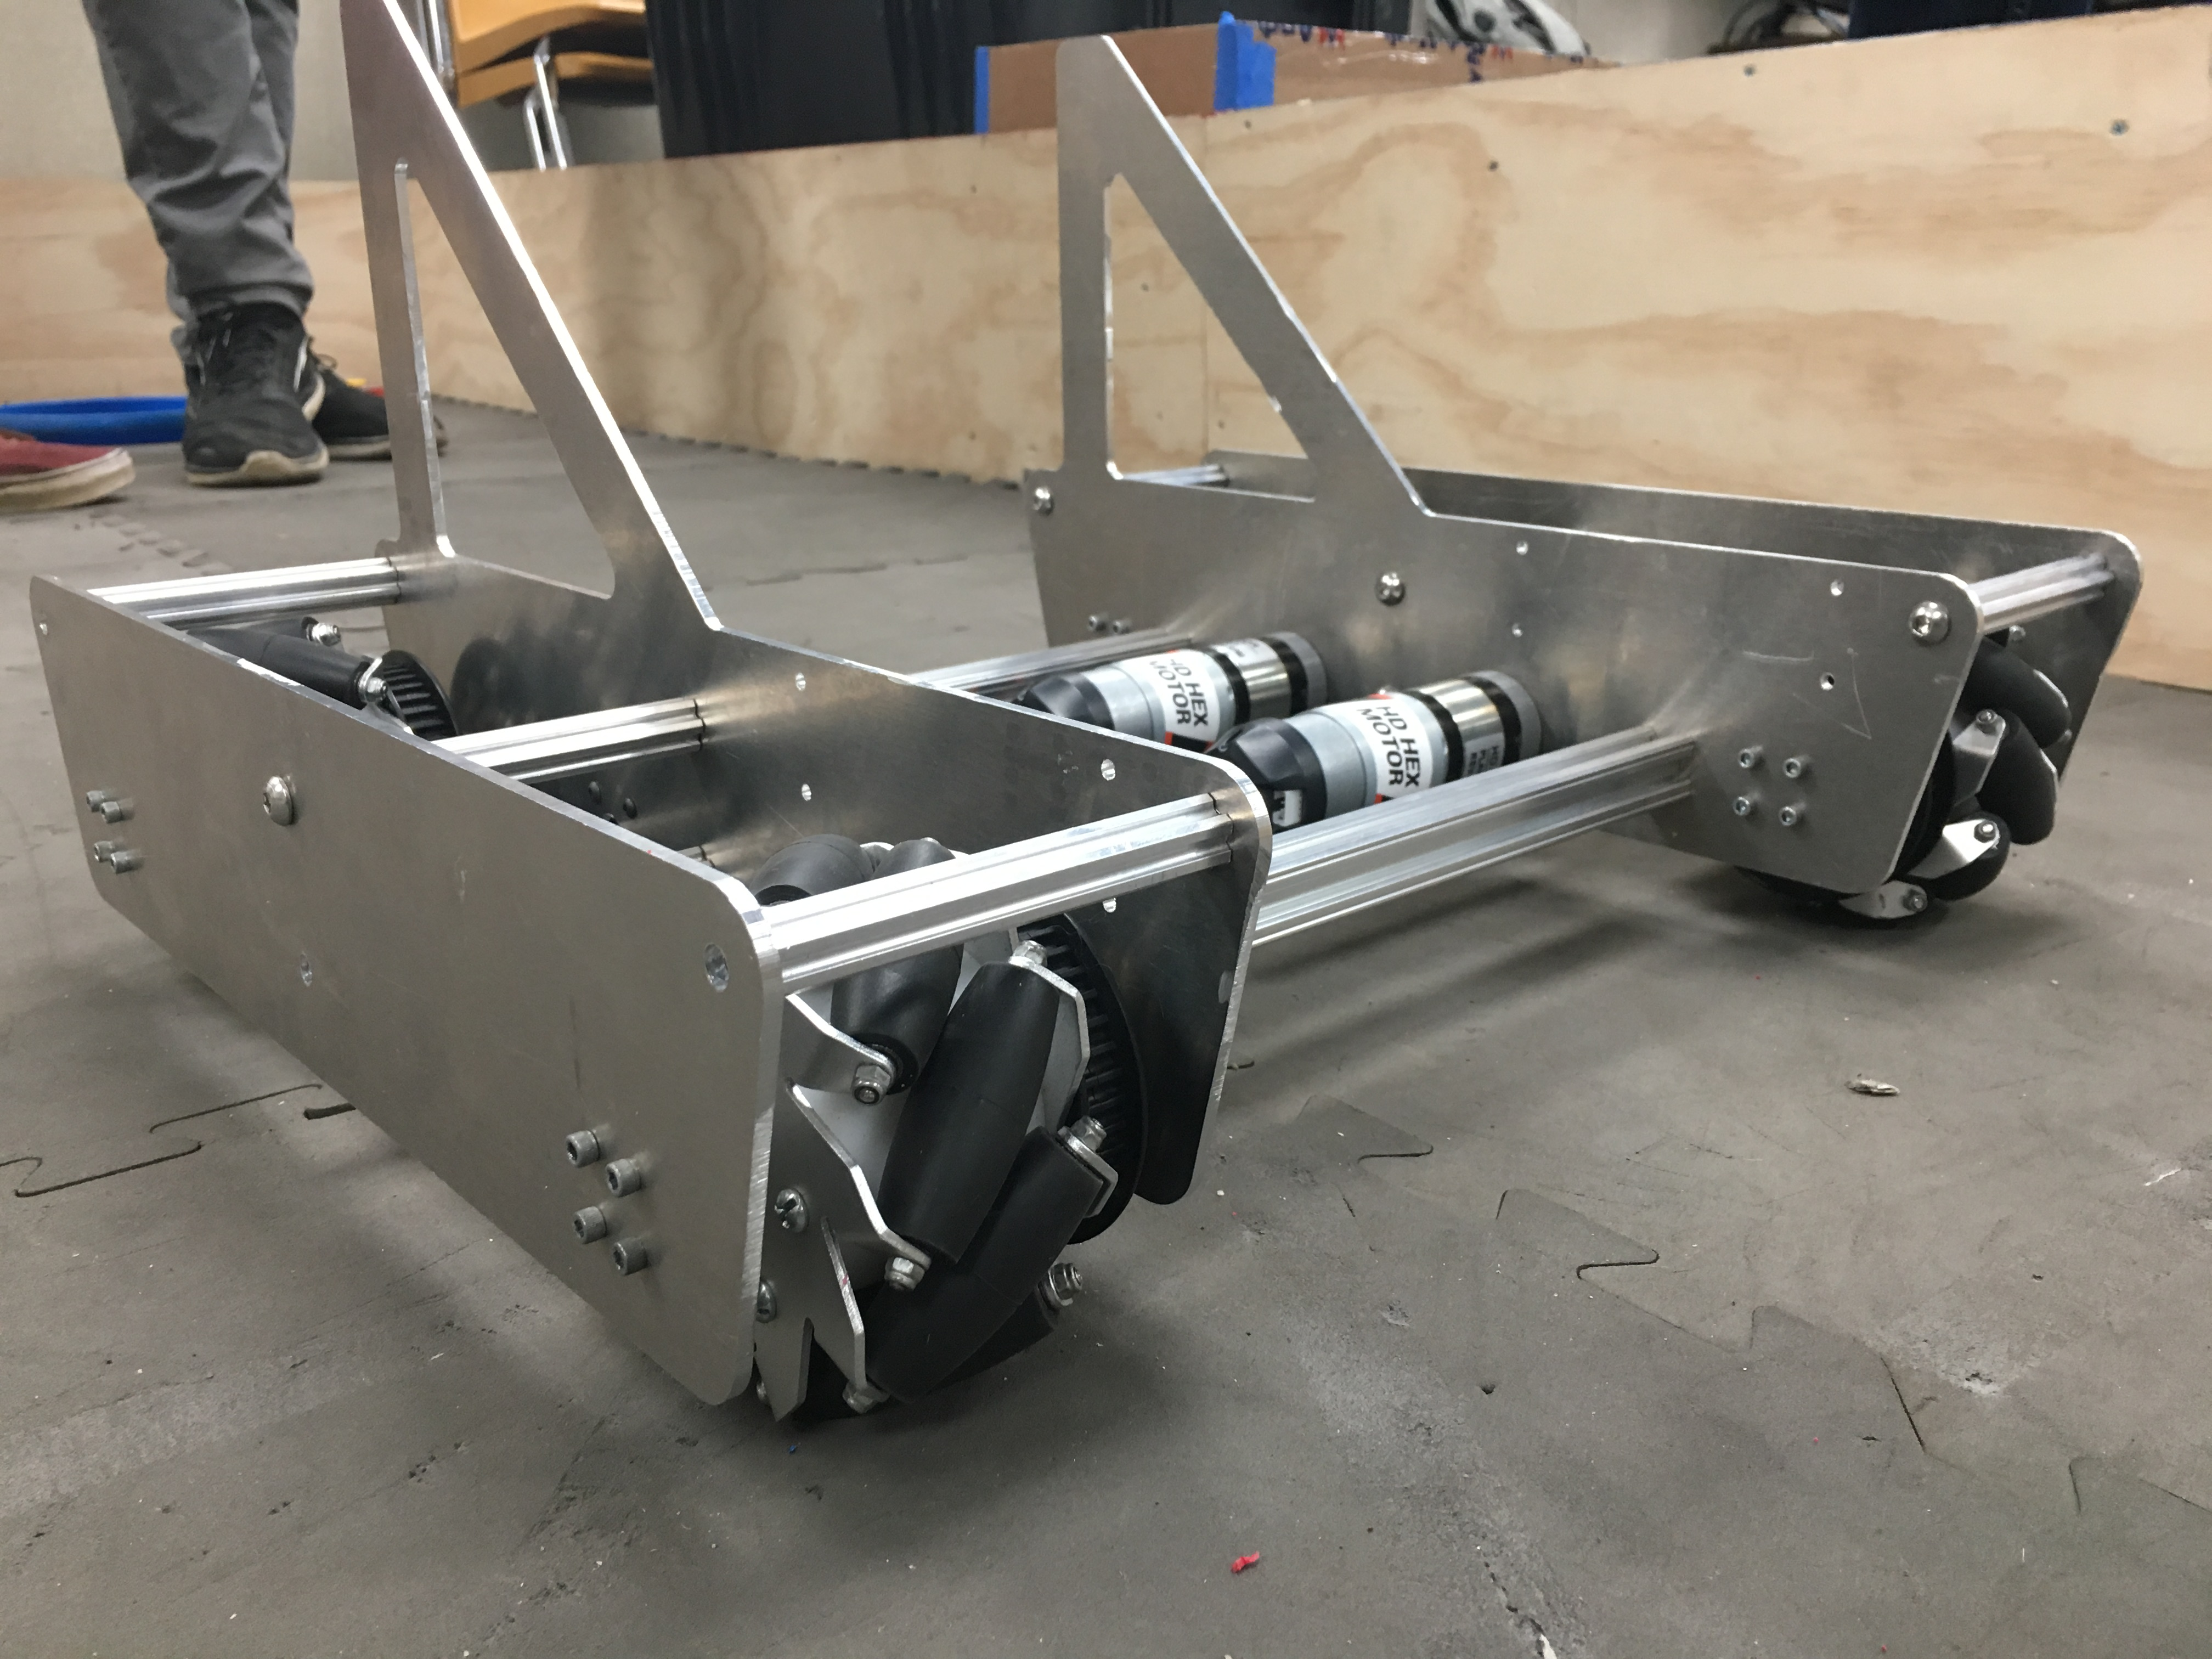
\includegraphics[width=.6 \textwidth]{10_11-05/images/drivetrain.JPG}
    \caption{Drivetrain}
    \label{fig:drivetrain}
\end{figure}

\end{document}